\section{Preliminaries}\label{sec:prel}

\subsection{Multisignatures}\label{sec:multisig}

A multisignature scheme~\cite{itakura1983public,CCS:MicOhtRey01} is a
tuple of algorithms:
$$
\ms = (\msSetup \times \allowbreak\msKeyGen \times \allowbreak\msCombVK \times \allowbreak
\msSign \times \allowbreak\msComb \times \allowbreak\msVfy)
$$
Where $\msSetup$ generates public parameters $\msParams$, such that
\begin{itemize}
  \item $(\msVK,\msSK) \gets \msKeyGen(\msParams)$ can be used to generate fresh key pairs,
  \item $\msSig \gets \msSign(\msParams,\msSK,\msMsg)$ signs  a message $\msMsg$ using key $\msSK$;
  \item $\msCSig \gets \msComb(\msParams,\msMsg,\msVKL,\msSigL)$ aggregates a
    set $\msSigL$ of signatures into a single, aggregate signature~$\msCSig$.
  \item $\msCVK \gets \msCombVK(\msParams,\msVKL)$ aggregates
  a tuple $\msVKL$ of verification keys $\msVK$ into a single,
  aggregate verification key $\msCVK$.
\end{itemize}
  $\msCVK$ can be used for verification:
  $\msVfy(\msParams,\msCVK,\msMsg,\msCSig) \in \{\true,\false\}$
  verifies an aggregate signature under an aggregate verification key.
  In the following, we often make the parameter~$\msParams$ implicit in the
    function calls for better readability.

  Intuitively, the security of a multisignature scheme guarantees
  that, if $\msCVK$ is produced from a tuple of verification keys
  $\msVKL$ via $\msCombVK$, then no aggregate signature $\msCSig$ can
  pass verification $\msVfy(\msCVK,\msMsg,\msCSig)$ unless all
  honest parties holding keys in $\msVKL$ signed $m$.

\begin{figure}[t]
  \centering
 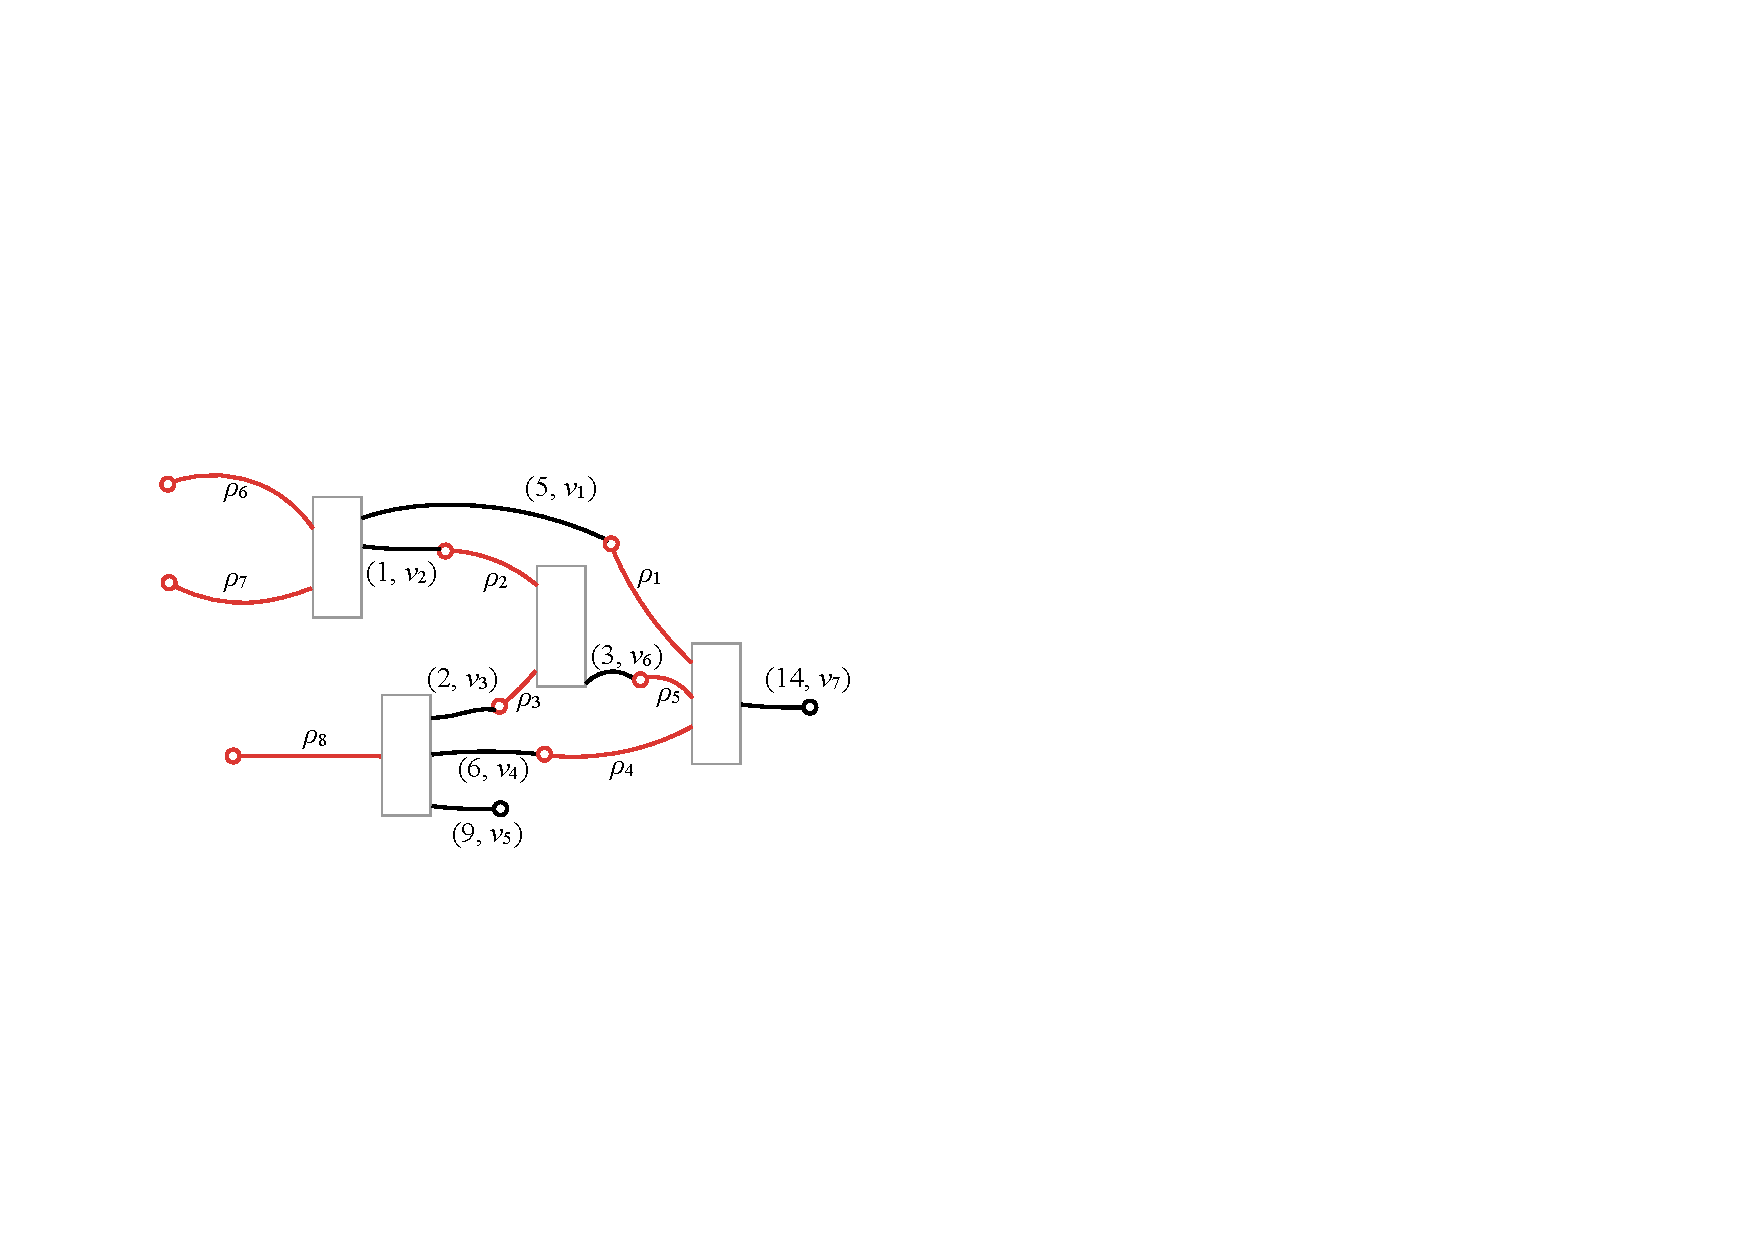
\includegraphics[width=\textwidth/2]{figures/utxo-graph.pdf}
 \caption{Example of a plain UTxO graph}
  \label{fig:utxo-graph}
\end{figure}

\subsection{Extended UTxO}
The basis for our fast isomorphic state channels is Bitcoin's UTxO ledger model~\cite{formal-model-of-bitcoin-transactions,Zahnentferner18-UTxO}. It arranges transactions in a directed acyclic graph structure, thus making the available parallelism explicit: 

\emph{Any two transactions that are not directly or indirectly dependent on each other can be processed independently.}

This arrangement results in graphs, such as the one in Figure~\ref{fig:utxo-graph},
where the boxes represent transactions with (red) inputs to the left and (black) outputs to the
right.

The set of dangling (unconnected) outputs are the \emph{unspent transaction outputs (UTxOs)} --- there are two of those in Figure~\ref{fig:utxo-graph}. 

\subsubsection{Notations}

In the rest of this document, we use of the following loosely specified functions and values: 
\begin{itemize}
   \item  $\mathbb{B} = \{0,1\}^k$ denotes a string of $k$ bits, eg. an arbitrary string of bytes, 
    \item $\mathbb{H} : \alpha \to \mathbb{B}$ denotes a \emph{hashing} function mapping arbitrary data to bytes, 
    \item $\mathsf{bits} : \alpha \to \mathbb{B}$ denotes an invertible \emph{serialisation} function mapping arbitrary data to bytes, 
    \item $k$, $k'$, $k_i$ denote \emph{verification keys},
   \item  $\mathcal{S}$ denotes the set of possible \emph{slot} values. 
\end{itemize}

\subsubsection{Definitions}

\begin{definition}[Value]

A \emph{value} $\mathsf{val}$ is a \emph{set} of \emph{tokens} represented as a tuple $(\mathsf{pid} \rightarrow \mathsf{tok} \rightarrow q)$ where
\begin{itemize}
    \item $\mathsf{pid} \in \{0,1\}^k$ is the \emph{Minting Policy identifier}, an arbitrary string of bytes corresponding to the \emph{hash} of a corresponding \emph{Minting Policy script},
    \item $\mathsf{tok} \in \{0,1\}^k$ is the \emph{Token name}, an arbitrary string of bytes,
    \item $q \in \mathbb{Z}$ is the quantity of this particular token.
\end{itemize}

\end{definition}

We use $\mathsf{Val}$ to denote the set of all possible values and  $\mu_x$ for minting policy scripts.

\begin{definition}[Validator Script]
A validator script $\nu$ is a pure function whose type is:
\[
  \nu : (\delta : \txDataTy) \to (\rho : \txDataTy) \to (\mathsf{tx} : \txPendingTxTy)
  \to\txBoolTy,
\]
where: 
\begin{itemize}
    \item $\txDataTy$ is a universal data type, and we denote an empty value of type $\txDataTy$ by $\emptyset$,  
    \item $\delta$ is the \emph{datum} part of the output to which this particular script is locked (see Definition \ref{def:outputs}),
    \item $\rho$ is the \emph{redeemer} provided as part of the transaction being validated,
    \item $\txBoolTy = \{\bot, \top\},$
    \item $\txPendingTxTy$ is the \emph{validation context}.
\end{itemize}
\end{definition}

Validator scripts are called \emph{phase-2} scripts in the Alonzo Ledger specification (see \cite{alozon-spec} for a formal treatment of these). Informally, scripts are \emph{evaluated} by the ledger when it \emph{applies} a transaction to its current state to yield a new ledger state. Each validator script referenced by an output is passed its arguments drawn from the output it locks and the transaction context it is executed in. The transaction is valid if and only if all scripts evaluates to $\top.$

We denote by $V$ the set of all validator scripts.

\begin{definition}[Outputs]
\label{def:outputs}
An \emph{output} $o$ is a triple $\mathsf{Val} \times V \times \txDataTy.$
We denote by $O$ the set of all possible outputs, and by $O_x$ the outputs in some context $x$.
\end{definition}

\begin{definition}[Inputs]
An input $i$ is pair $(\txOutRef, \rho)$ where 
$\txOutRef \in (\mathsf{TxId} \times \mathbb{N})$ is the input reference with $\mathsf{TxId} \subseteq \mathbb{B},$ and $\rho \in \txDataTy$ is the \emph{input}'s redeemer.  We denote by $I$ the set of all possible inputs, and by $I_x$ the outputs in some context $x$.
\end{definition}

\begin{definition}[Validation Context]

A validation context $\txPendingTx$ is a tuple  
$$(I_\sigma, O_\sigma, \mathsf{Mint}, \txRmin, \txRmax, \txKeys)$$
where:
\begin{itemize}
    \item $I_\sigma \in I^w$ is a list of inputs of length $w$,
    \item $O_\sigma \in O^y$ is a list of outputs of length $y$,
    \item $\mathsf{Mint} \subset \mathsf{Val}$ is the \emph{Minted} values,
    \item $(\txRmin, \txRmax) \in \mathcal{S} \times \mathcal{S}$ are the lower and upper validity bounds of the enclosing transaction,
    \item $\txKeys$ is the set of public keys signing the enclosing transaction.
\end{itemize}

\end{definition}

\subsection{State Machines}
%\label{sec:state_machines}
A convenient abstraction for EUTxO smart contracts spanning a sequence
of related transactions are state machines. Specifically, we adopt
\emph{constraint emitting machines (CEMs)}~\cite{eutxo}. These are
based on Mealy machines and consist of a set of states $\cemS$, a set
of inputs $\cemI$, a predicate \(\cemFinal : \cemS\to\txBoolTy\)
identifying final states, and a step relation
\(\cemStepRel{s}{i}{s'}{\cemTxCon}\), which takes a state $s$ on an
input $i$ to a successor state $s'$ under the requirements that the
constraints $\cemTxCon$ are satisfied.

We implement CEMs on a EUTxO ledger (the mainchain) by representing a sequence of CEM states as a sequence of transactions. Each of these transactions has got a \emph{state-machine input} $\cemIn$ and a \emph{state-machine output} $\cemOut$, where the latter is locked by a validator $\cemVal$, implementing the step relation. The only exceptions are the initial and final state, which have got no state-machine input and output, respectively.

\begin{figure}[t]
  \centering
  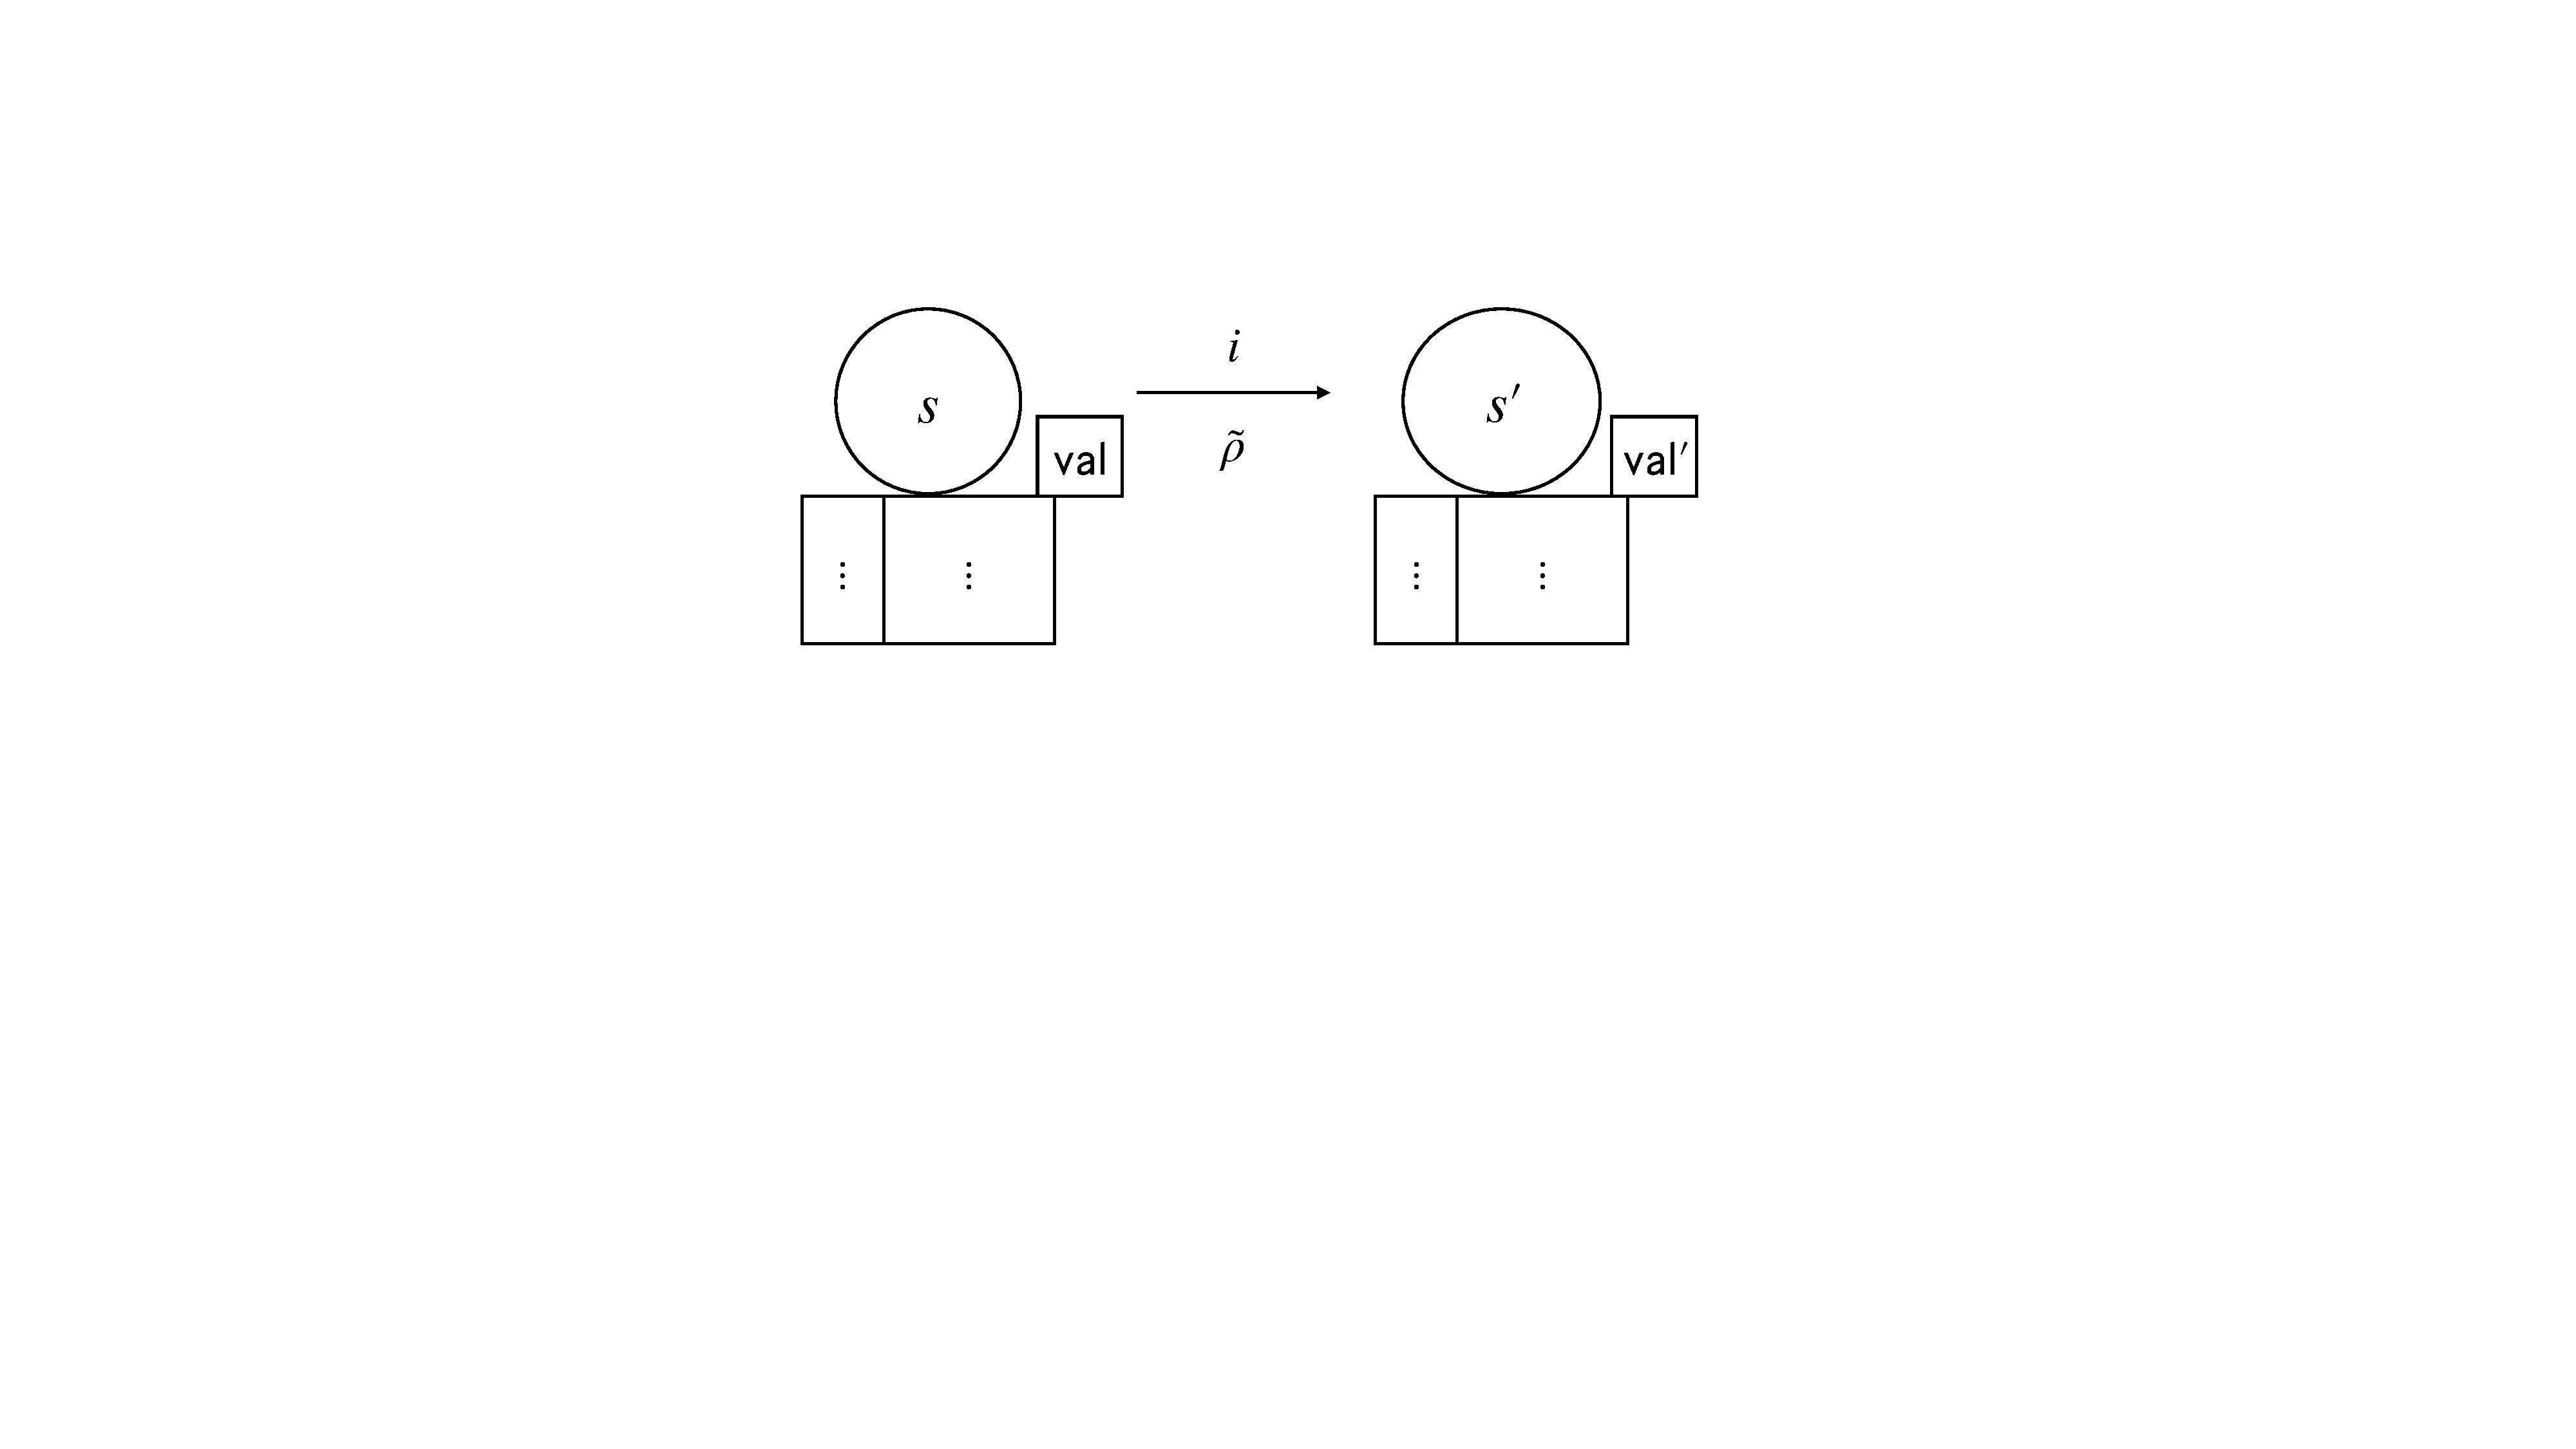
\includegraphics[scale=.2,width=\textwidth/2]{figures/state-transition_cropped.pdf}
  \caption{Transactions representing successive states in a CEM
    transition relation \(\cemStepRel{s}{i}{s'}{\cemTxCon}\).  Fields
    $\val$ and $\val'$ are the value fields of the state-machine
    outputs and $\tilde \rho$ is the additional data.}
  \label{fig:state-transition}
\end{figure}

More specifically, given two transactions $\tx$ and $\tx'$, they represent successive states under \(\cemStepRel{s}{i}{s'}{\cemTxCon}\) iff 

\begin{mitemize}
  \item state-machine output $\cemOut = (\txVal, \cemVal, s)$ of $\tx$
  is consumed by the state-machine input $\cemIn' = (\txOutRef, \rho)$
  of $\tx'$, whose redeemer is \(\rho = i\) (i.e., the redeemer
  provides the state-machine input) and
  \item either $\cemFinal(s') = \true$ and $tx'$ has no state-machine
  output, or $\cemOut' = (\txVal', \cemVal, s')$ and $\tx'$ meets all
  constraints imposed by $\cemTxCon$.
\end{mitemize}
Sometimes it is useful to have additional data $\tilde \rho$ provided
as part of the redeemer, i.e., $\rho = (i,\tilde \rho)$.

A state transition of the described type is represented by two connected
transactions as shown in Fig.~\ref{fig:state-transition}.  For
simplicity, state-machine inputs and outputs are not shown, with the
exception of the value fields $\txVal$ and $\txVal'$ of the state-machine output.


%%% Local Variables:
%%% mode: latex
%%% TeX-master: "main"
%%% End:
